\section{作业及答案：结构力学基础与技巧班第4次作业及答案（静定梁和刚架）}
\begin{analysisbox}
静定结构按平衡方程逐段推进即可。集中力使剪力突变，集中力矩使弯矩突变，均布荷载区段的剪力为一次函数、弯矩为二次函数。
\end{analysisbox}
\subsection*{第 1 页转写}
结力基础班第4次作业

梁和刚架

梁和刚架作业及答案

图2-60所示结构截面A的弯矩（以下侧受拉为正）是（

2-1

）。（西南交通大学

2008)

A. M

B. -M

C. -2M

D. 0

2-2图2-61所示结构剪力FQBA=

（重庆大学2010）

图2-60

图2-61

剪力为

图2-62所示刚架中AB杆的弯矩为

2-3

（河北工业大学

2010)

2-4图2-63所示刚架，AD杆截面D弯矩MDA=

（内侧受拉为正）。（浙江

大学2011)

10kN-m

30kN

5kN-m

4m

8m

图2-62

图2-63

2-5试作图2-64所示结构的弯矩图。（北京科技大学2008)

2-6作图2-65所示多跨梁的弯矩图和剪力图，并给出AB杆的受力平衡图。（北京

交通大学2011)

10kN

20kN

4kN

6kN/m

40kN-m

10kN/m

2m

2m

12mJ

8x2m

2m

图2-64

图2-65
\begin{figure}[H]\centering
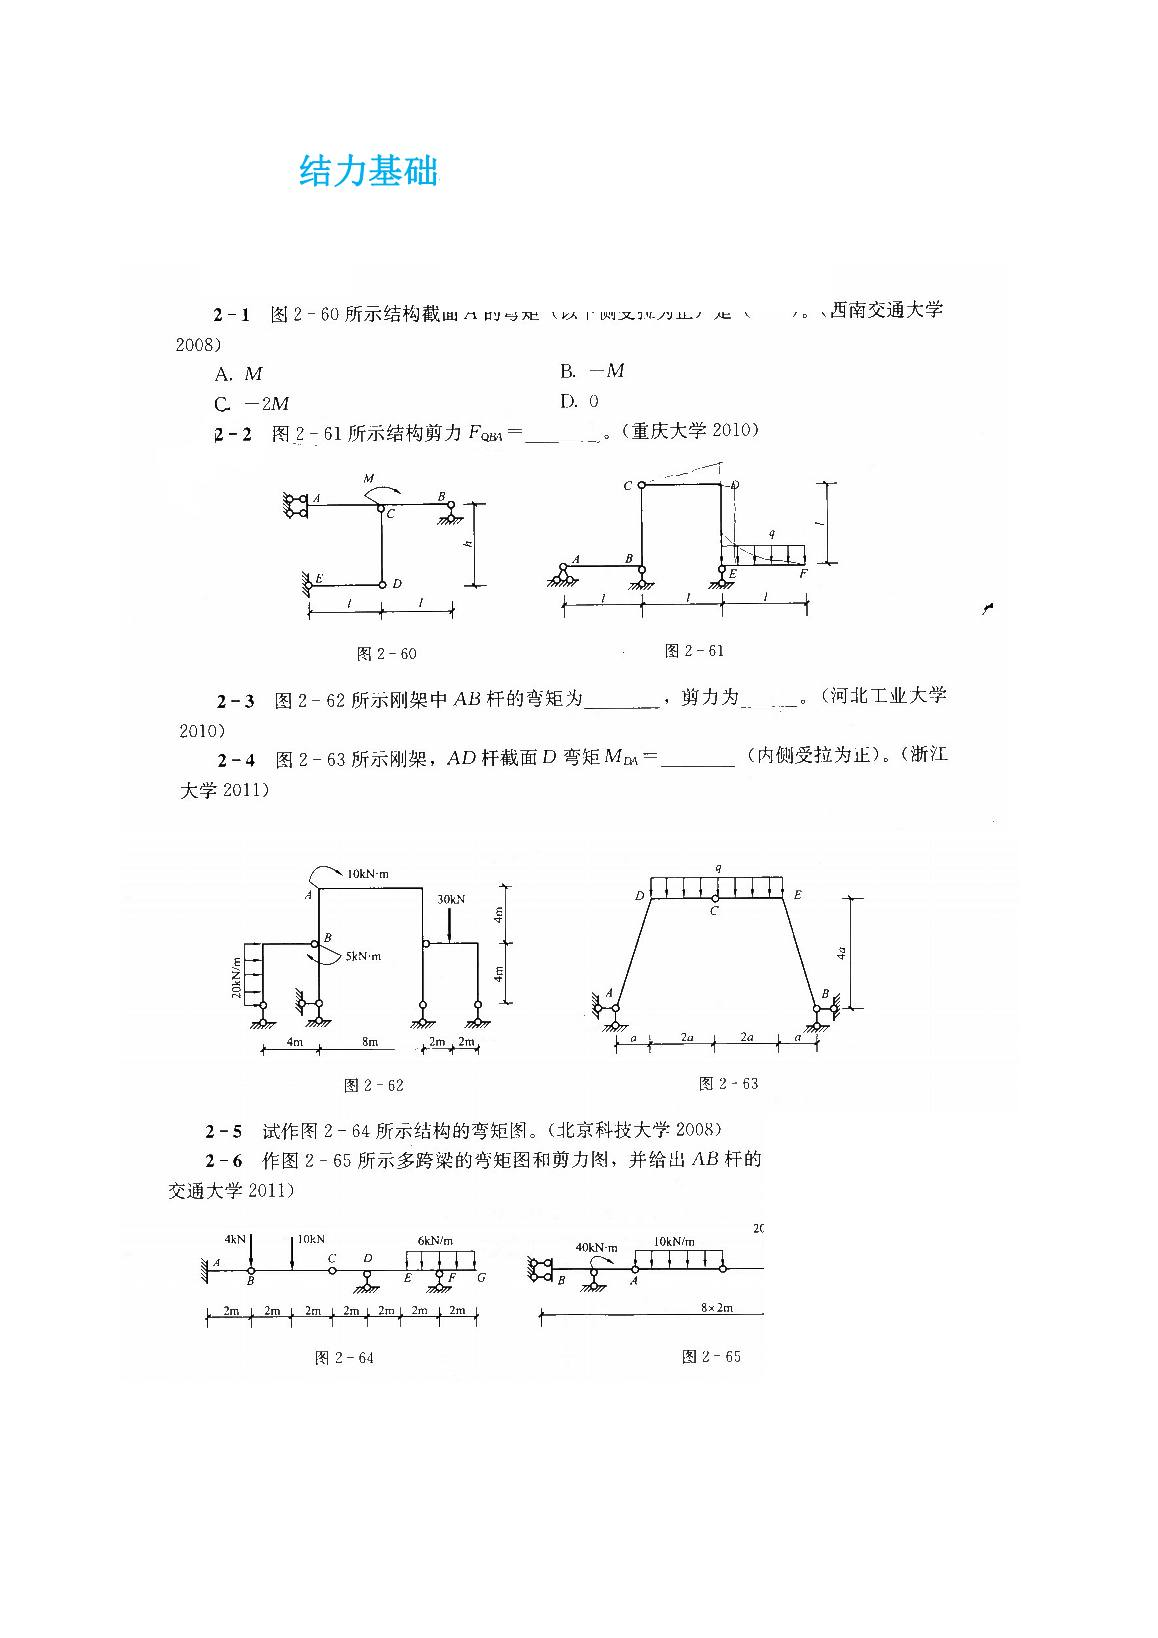
\includegraphics[width=0.92\textwidth]{figures/src07_p001.jpg}
\caption{结构力学基础与技巧班第4次作业及答案（静定梁和刚架） 第 1 页清理图形页}
\end{figure}
\subsection*{第 2 页转写}
2-7求图2-66所示结构的内力、作弯矩图（可不写过程）。（东南大学2008）

2-8

绘出图2-67所示结构的弯矩图。（武汉大学2010）

40k

40kN

40kN/m

图2-66

图2-67

.2-g

作图2-68所示静定刚架M图。（福州大学2008）

2-10

绘制图2-69所示结构的弯矩图。（武汉科技大学2g995

/m

20kN

kN/m

3kN-m

2m

3m

(图2-68

图2-69

2-11

绘图2－70所示结构的弯矩图。（重庆大学2012）

/2-12已知图2-71所示结构的弯矩图，试作剪力图和轴力图。已知Fp=10kN，M=

40kN m。（哈尔滨工业大学2010）

40

M图(kN-m)

2m

2m

20

图2-7

2 -13

作图2-72所示刚架的弯矩图。（中南大学2009）

2 - 14

绘出图2－73所示结构的弯矩图。（武汉大学2010）

Fp=q!

2kN/m

4kN-m

3kN

2m

2m

图2-72

图2-73
\begin{figure}[H]\centering
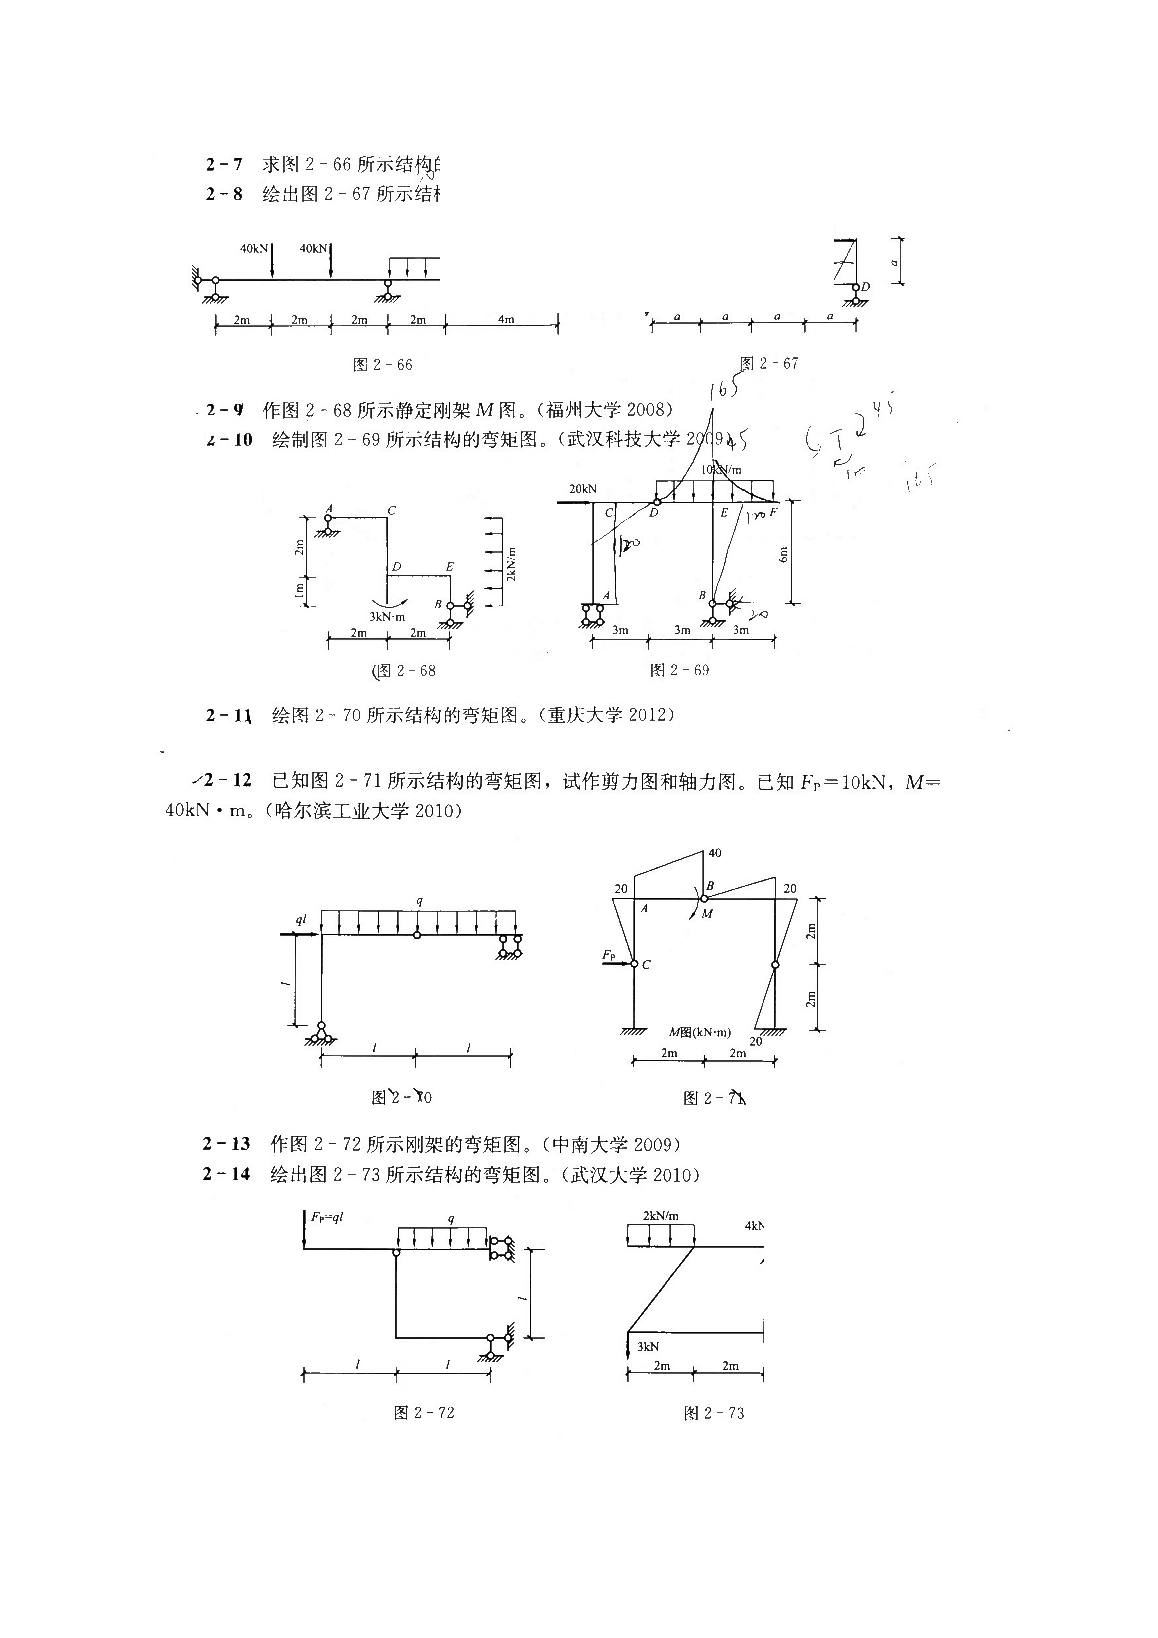
\includegraphics[width=0.92\textwidth]{figures/src07_p002.jpg}
\caption{结构力学基础与技巧班第4次作业及答案（静定梁和刚架） 第 2 页清理图形页}
\end{figure}
\subsection*{第 3 页转写}
2-15

作图2－74所示结构的内力图。（北京工业大学2011）

2-16

求图2－75所示结构的内力，并作弯矩图。（可不写过程）（东南大学2008）

30kN-m

10kN

30kN

8m

图2-74

图2-75

2-17

作图2－76所示结构的弯矩图。（无须写出分析过程）（东南大学2007）

2-18

作图2-77所示结构弯矩图。（中南大学2010）

10kN/m

20kN/m

30kN

40kN

图2-76

图2-

2 -19

已知结构在集中力和集中力偶矩作用下的弯矩图如图2－78所示，其中BC段

为二次抛物线，试确定结构所受的荷载情况，并绘出BE段隔离体受力平衡图。（北京交通

大学2009)

2-20已知图2-79所示静定刚架的弯矩图（曲线部分为二次抛物线），试绘图标出作

用于刚架上的荷载，并作出剪力图和轴力图（假设各杆无局部平衡的轴向荷载，无分布力

偶）。（浙江大学2012）

3qq2

pbz

M图(kN m)

2m

2m

图2-78

图2-79
\begin{figure}[H]\centering
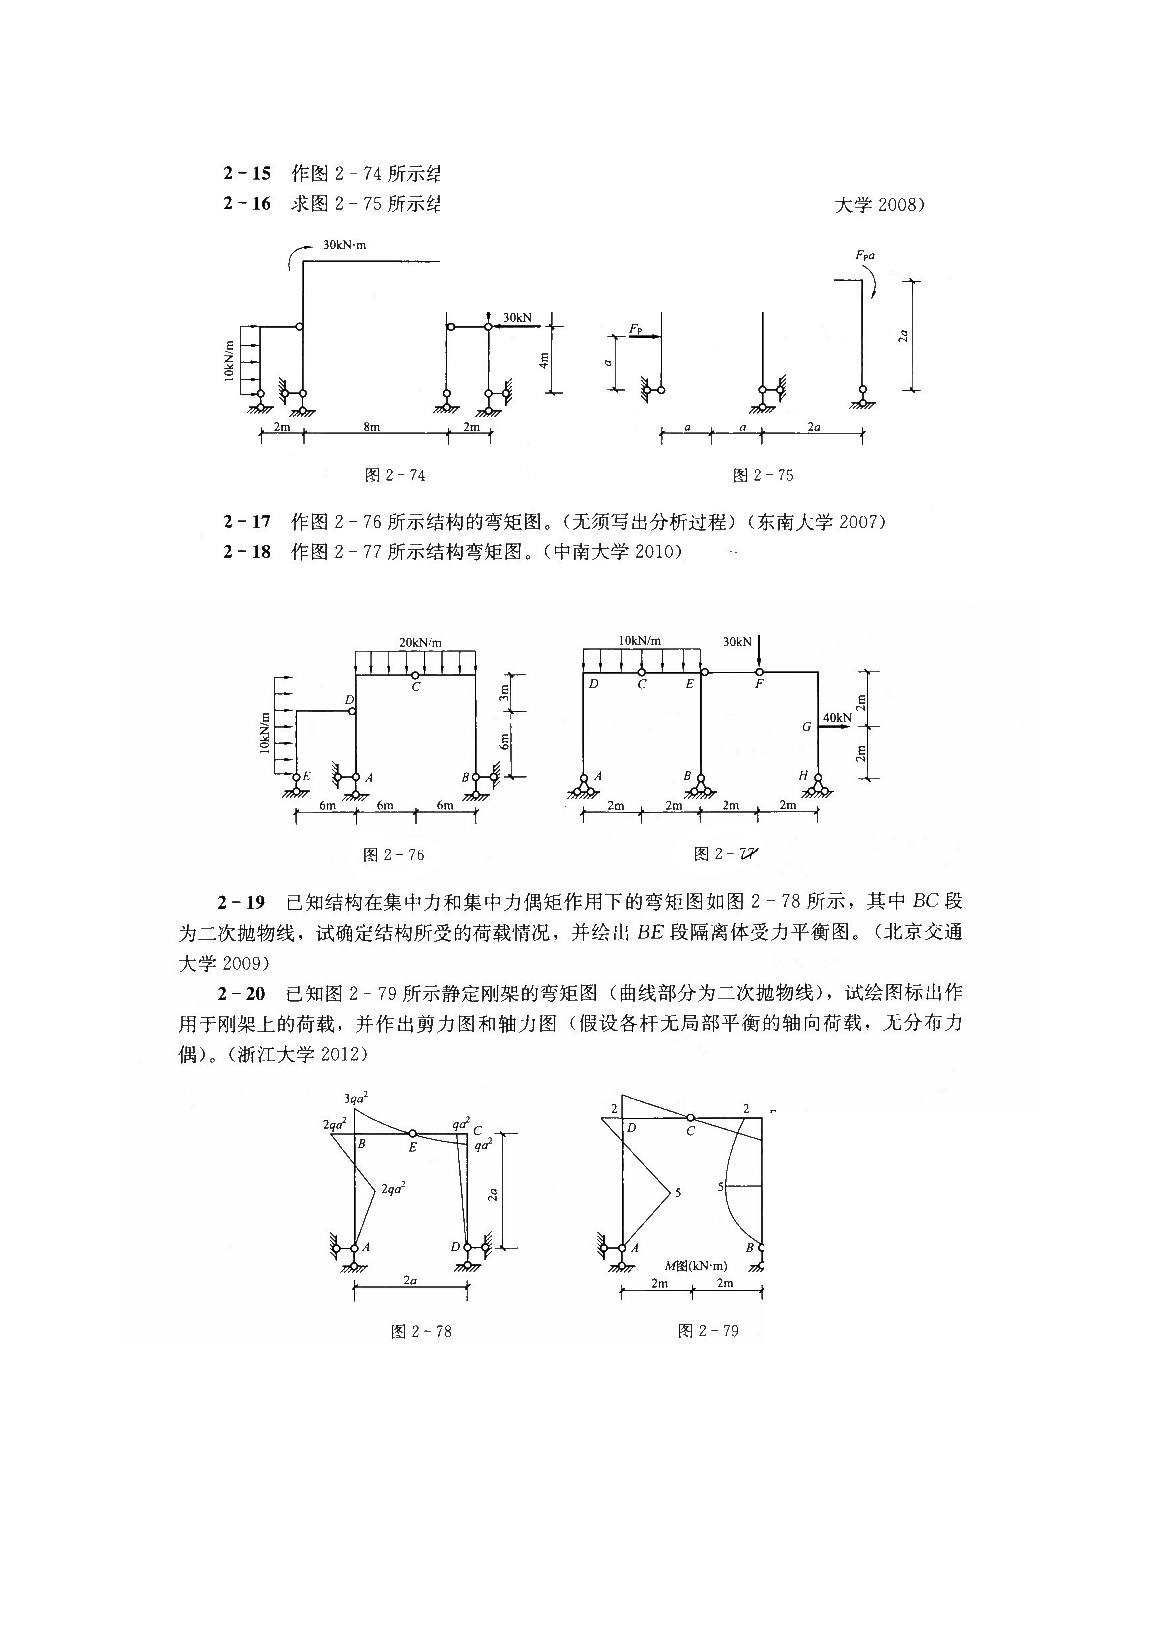
\includegraphics[width=0.92\textwidth]{figures/src07_p003.jpg}
\caption{结构力学基础与技巧班第4次作业及答案（静定梁和刚架） 第 3 页清理图形页}
\end{figure}
\subsection*{第 4 页转写}
2-21不经过计算，绘制图2-80所示结构弯矩图。（武汉科技大学2009）

2-22试求解图2-81所示刚架，并绘制弯矩图。（东北大学2005）

FP

10kN-m

3m

3m

5m

3m

3m

图2-80

图2-8Y
\begin{figure}[H]\centering
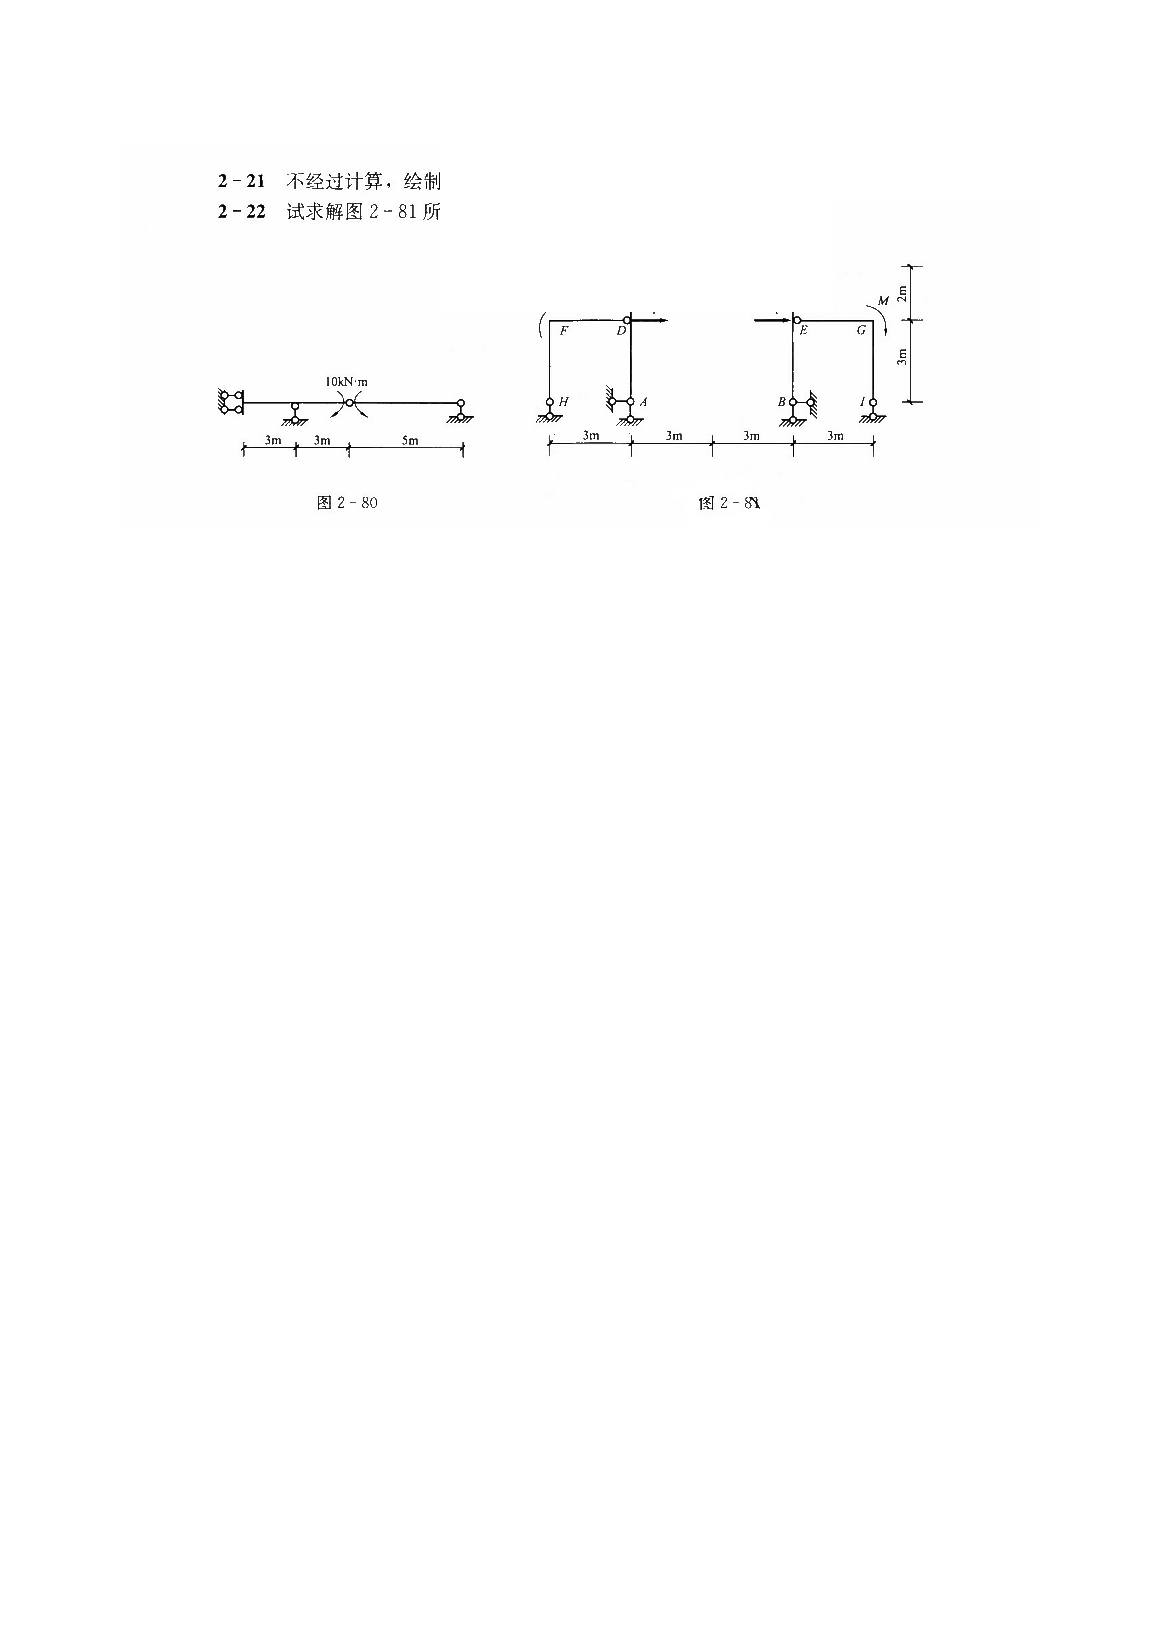
\includegraphics[width=0.92\textwidth]{figures/src07_p004.jpg}
\caption{结构力学基础与技巧班第4次作业及答案（静定梁和刚架） 第 4 页清理图形页}
\end{figure}
\subsection*{第 5 页转写}
22.

QBA-O.

2-31

EX70,FxL=x4=10y

Mes: x 44e 1bo kwm

MF=Mj 4$\times$ 30x4=30k.m

MB=

Tay$\times$ 4= 2x4x 2 Fay= 40kv

40.
\begin{figure}[H]\centering
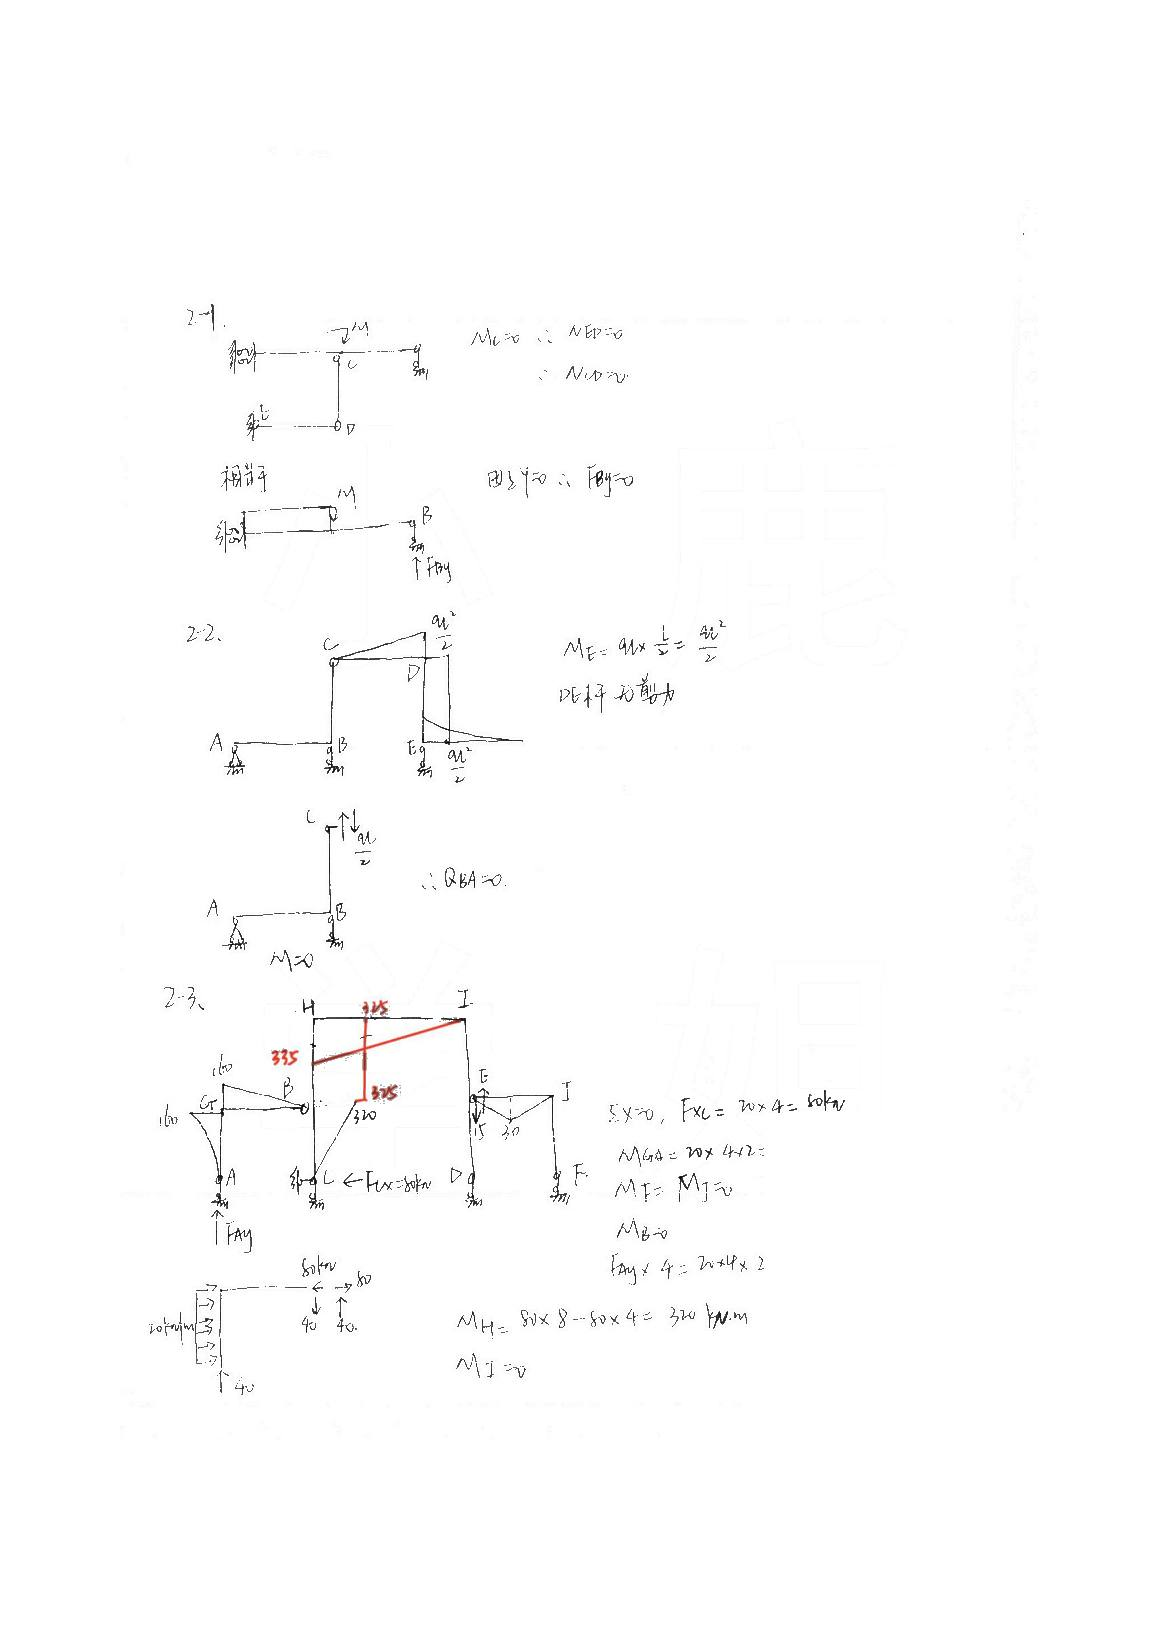
\includegraphics[width=0.92\textwidth]{figures/src07_p005.jpg}
\caption{结构力学基础与技巧班第4次作业及答案（静定梁和刚架） 第 5 页清理图形页}
\end{figure}
\subsection*{第 6 页转写}
2-4

MA0.

Fyp$\times$b4=9$\times$ 40$\times$39

TyB= 240

FxBx4a+9x24$\times$a=4x30

Txb= 90.

0-94$\times$4-244$\times$4=22（例受拉）

18

B为阳属

Fp$\times$ 4=5x 6

40

10$\times$40

MD= 70x 4+ 70x 2 20xb= 170 kvm
\begin{figure}[H]\centering
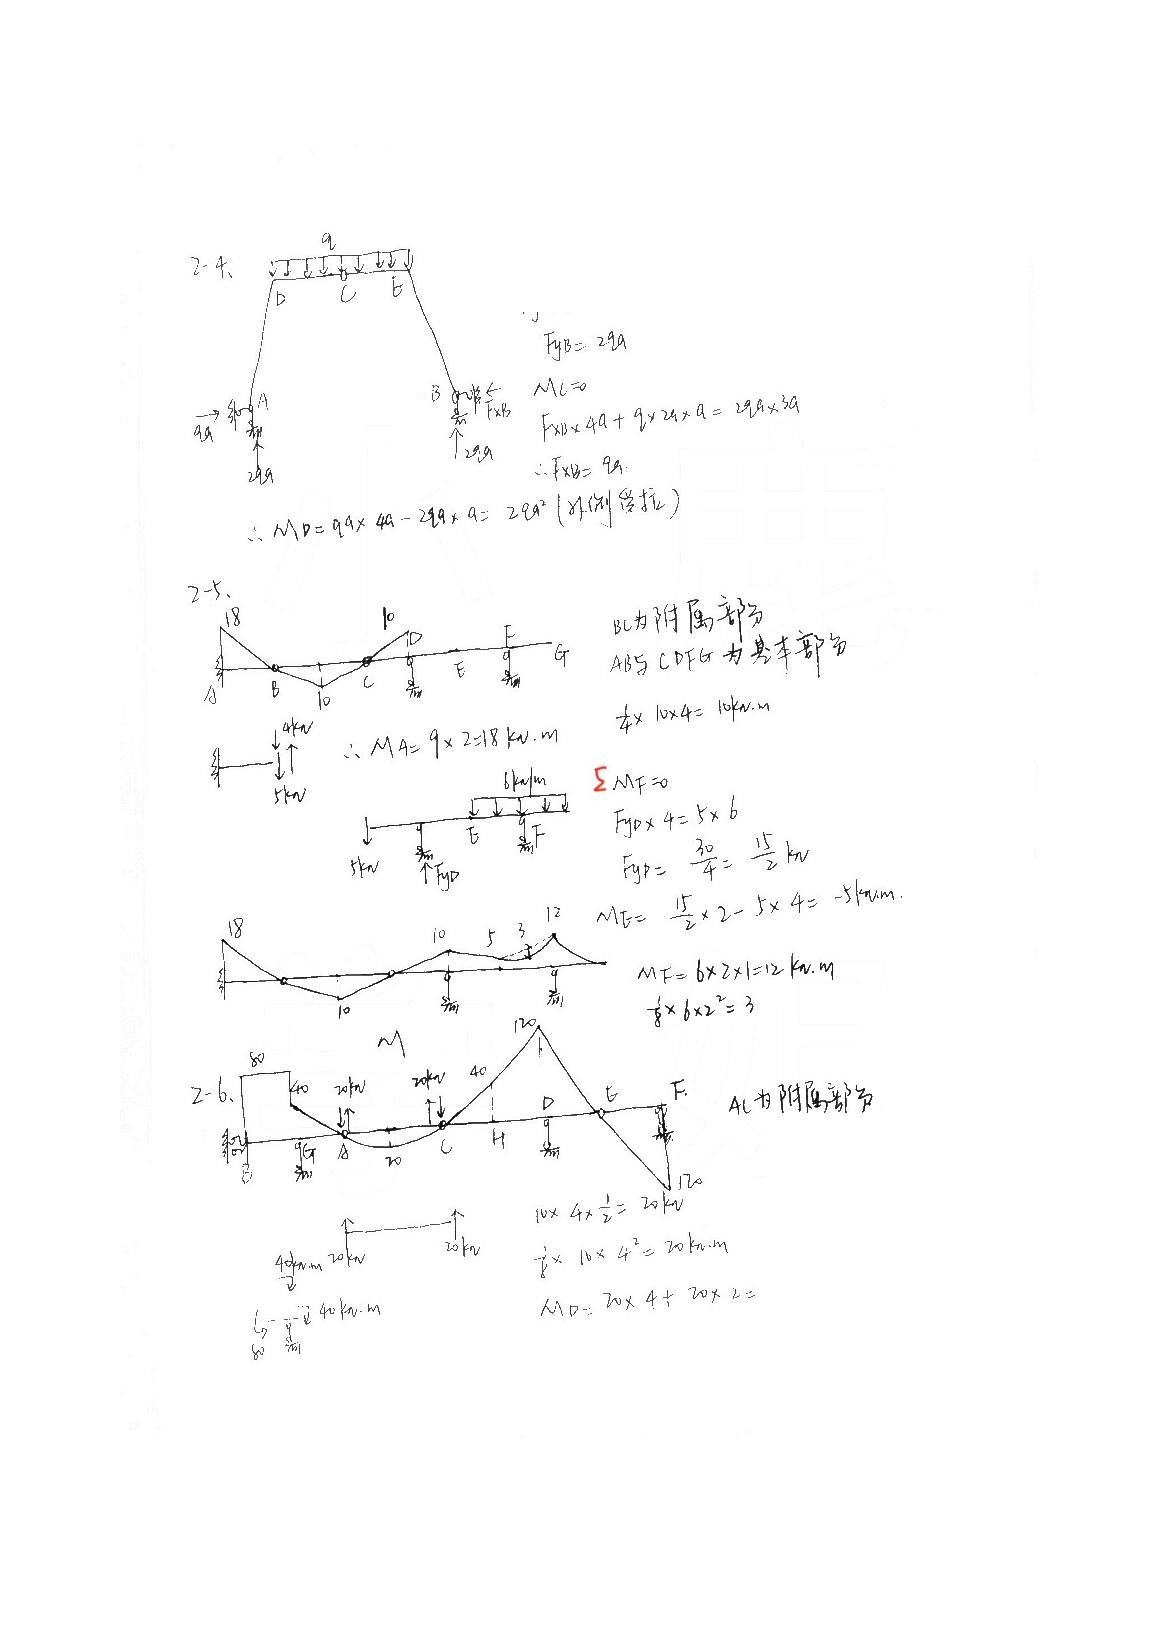
\includegraphics[width=0.92\textwidth]{figures/src07_p006.jpg}
\caption{结构力学基础与技巧班第4次作业及答案（静定梁和刚架） 第 6 页清理图形页}
\end{figure}
\subsection*{第 7 页转写}
A嘟用音如法

MB=\&0x240x2l240kv.m

40

40

4d

个40

2-8

MA= 2xG-Fpx=Fr9

Fy4x 4= 3+ 2xx

TBx= 2x3= 6 kv
\begin{figure}[H]\centering
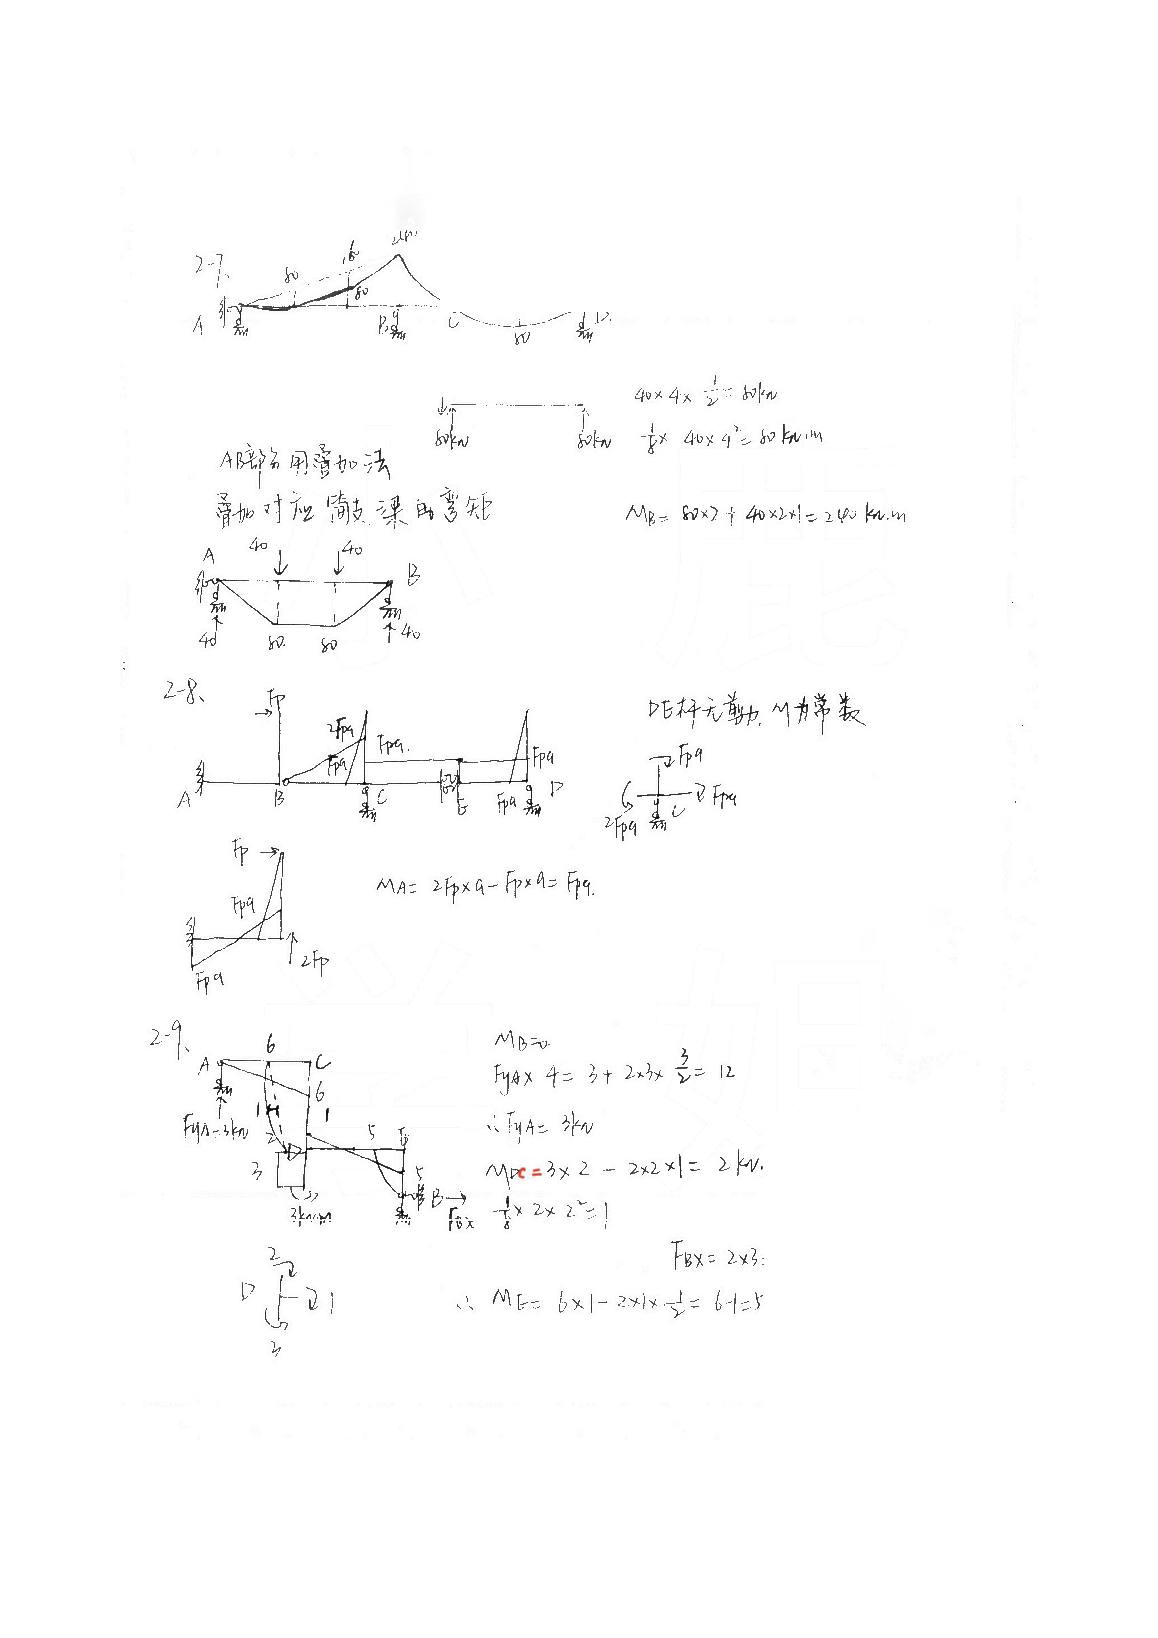
\includegraphics[width=0.92\textwidth]{figures/src07_p007.jpg}
\caption{结构力学基础与技巧班第4次作业及答案（静定梁和刚架） 第 7 页清理图形页}
\end{figure}
\subsection*{第 8 页转写}
170

10x3$\times$=4h

ME0 165

B4

10x3x\#+ Fapx 3=165

no

10

个个个

MB=

40

212
\begin{figure}[H]\centering
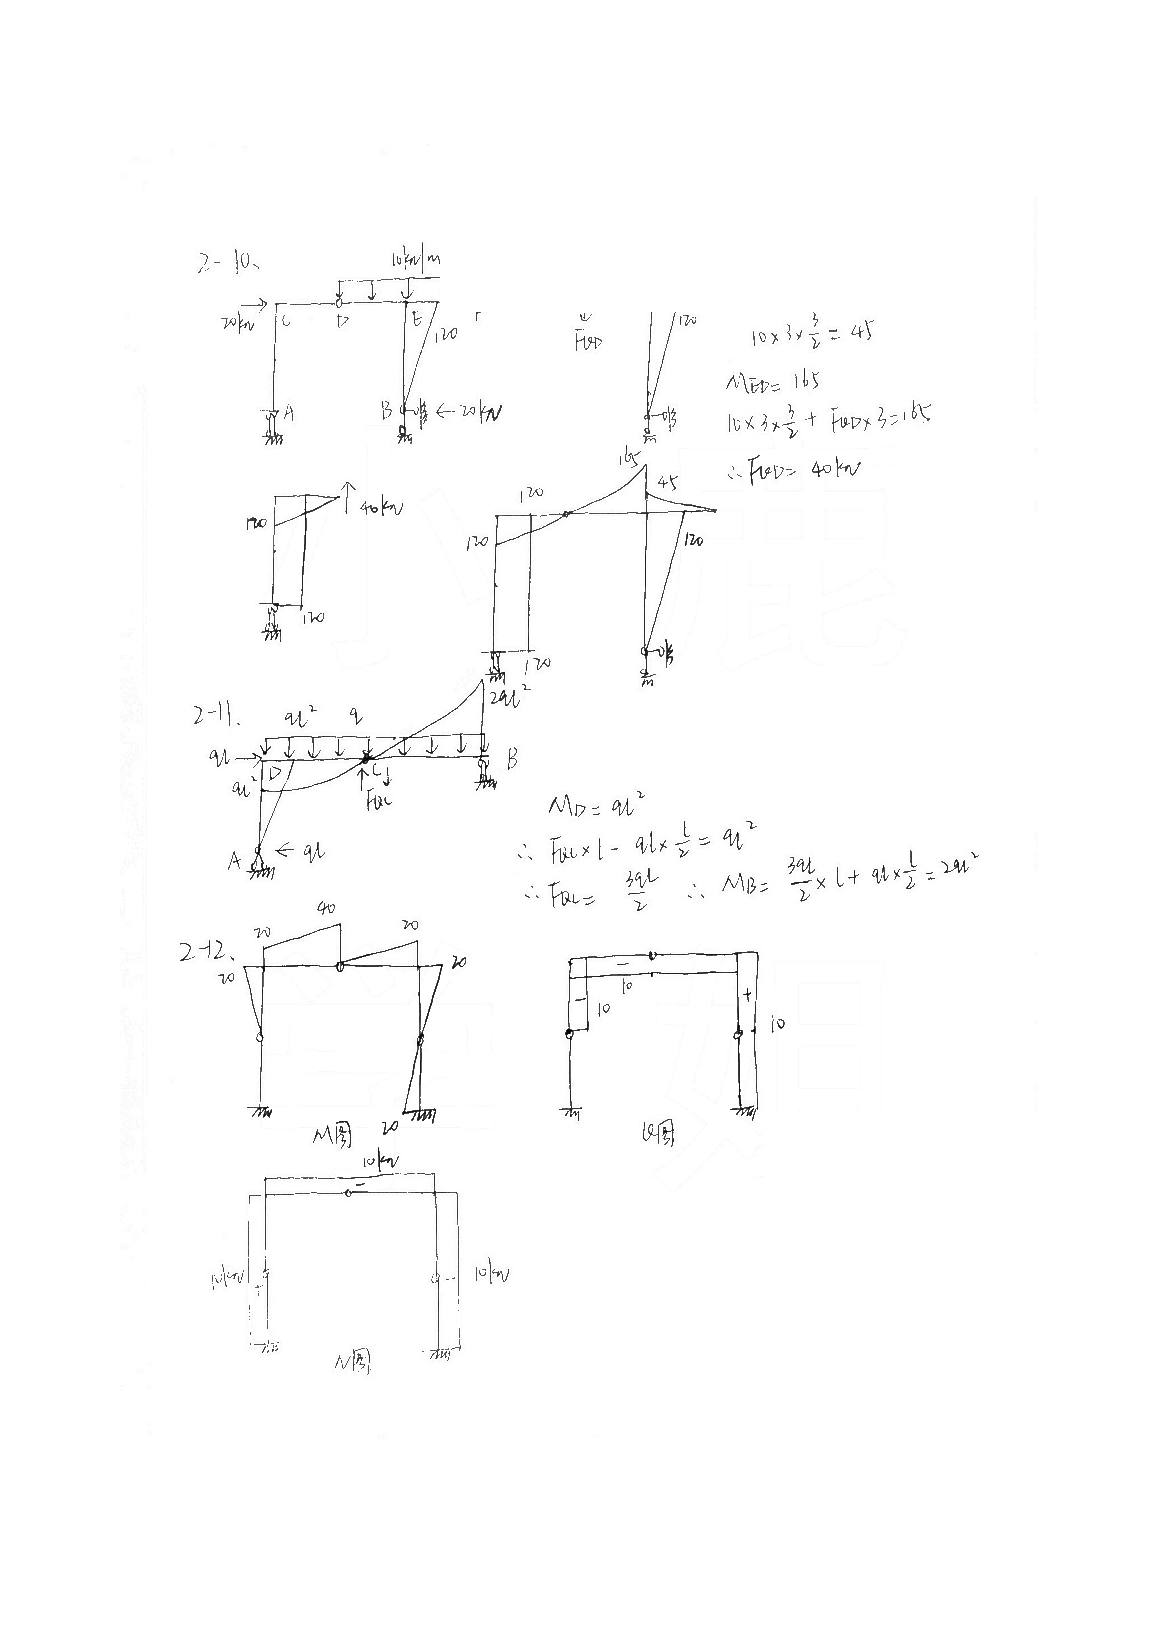
\includegraphics[width=0.92\textwidth]{figures/src07_p008.jpg}
\caption{结构力学基础与技巧班第4次作业及答案（静定梁和刚架） 第 8 页清理图形页}
\end{figure}
\subsection*{第 9 页转写}
2912

214

2424 1=4

M3= 4+ 22+/=8

Mc 3$\times$4+ 2x2$\times$3- 4= 20

30kv-m

2 -15,

MA-KBXFO

80
\begin{figure}[H]\centering
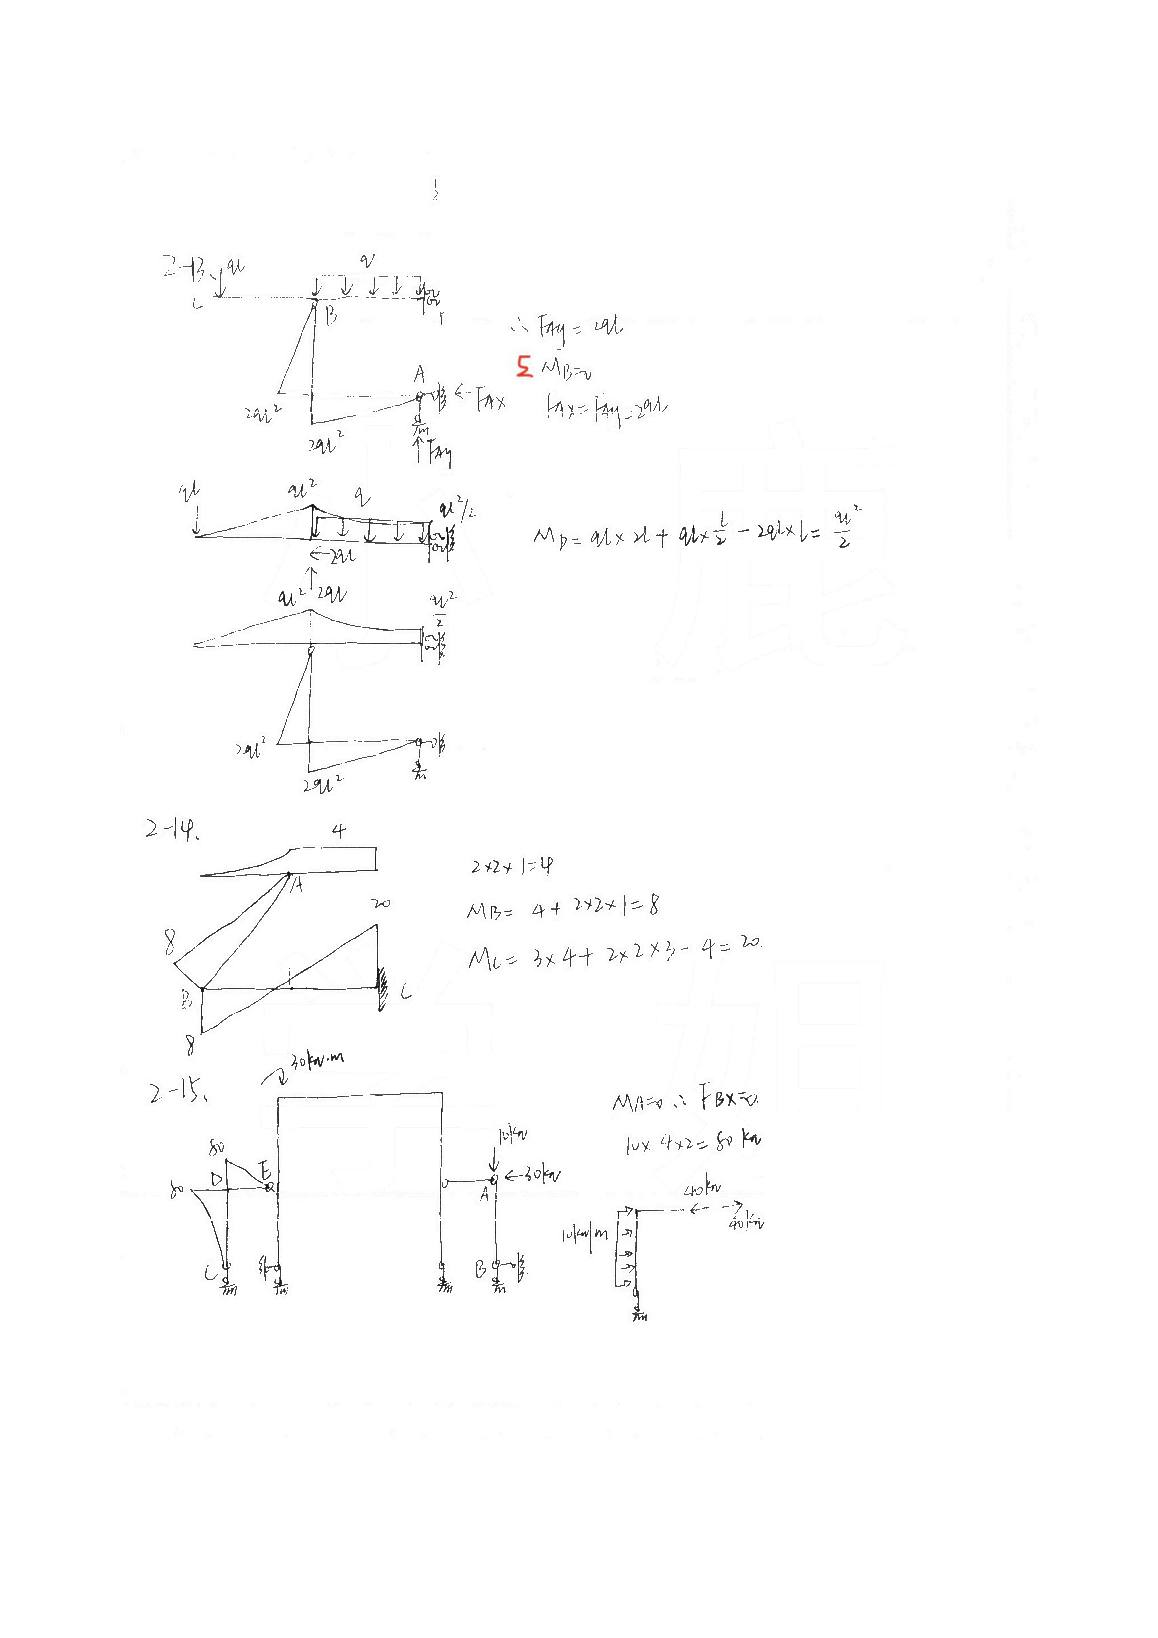
\includegraphics[width=0.92\textwidth]{figures/src07_p009.jpg}
\caption{结构力学基础与技巧班第4次作业及答案（静定梁和刚架） 第 9 页清理图形页}
\end{figure}
\subsection*{第 10 页转写}
=8 X X=8XaXob

M fu= 40x 4\textasciitilde{} 10x 8= 80 kv.my.

20

40

08

8.75

30

40

30

8.75

30

40

40

8.75

10

10

40

48.75

FQ图(kN)

FN图(kN)
\begin{figure}[H]\centering
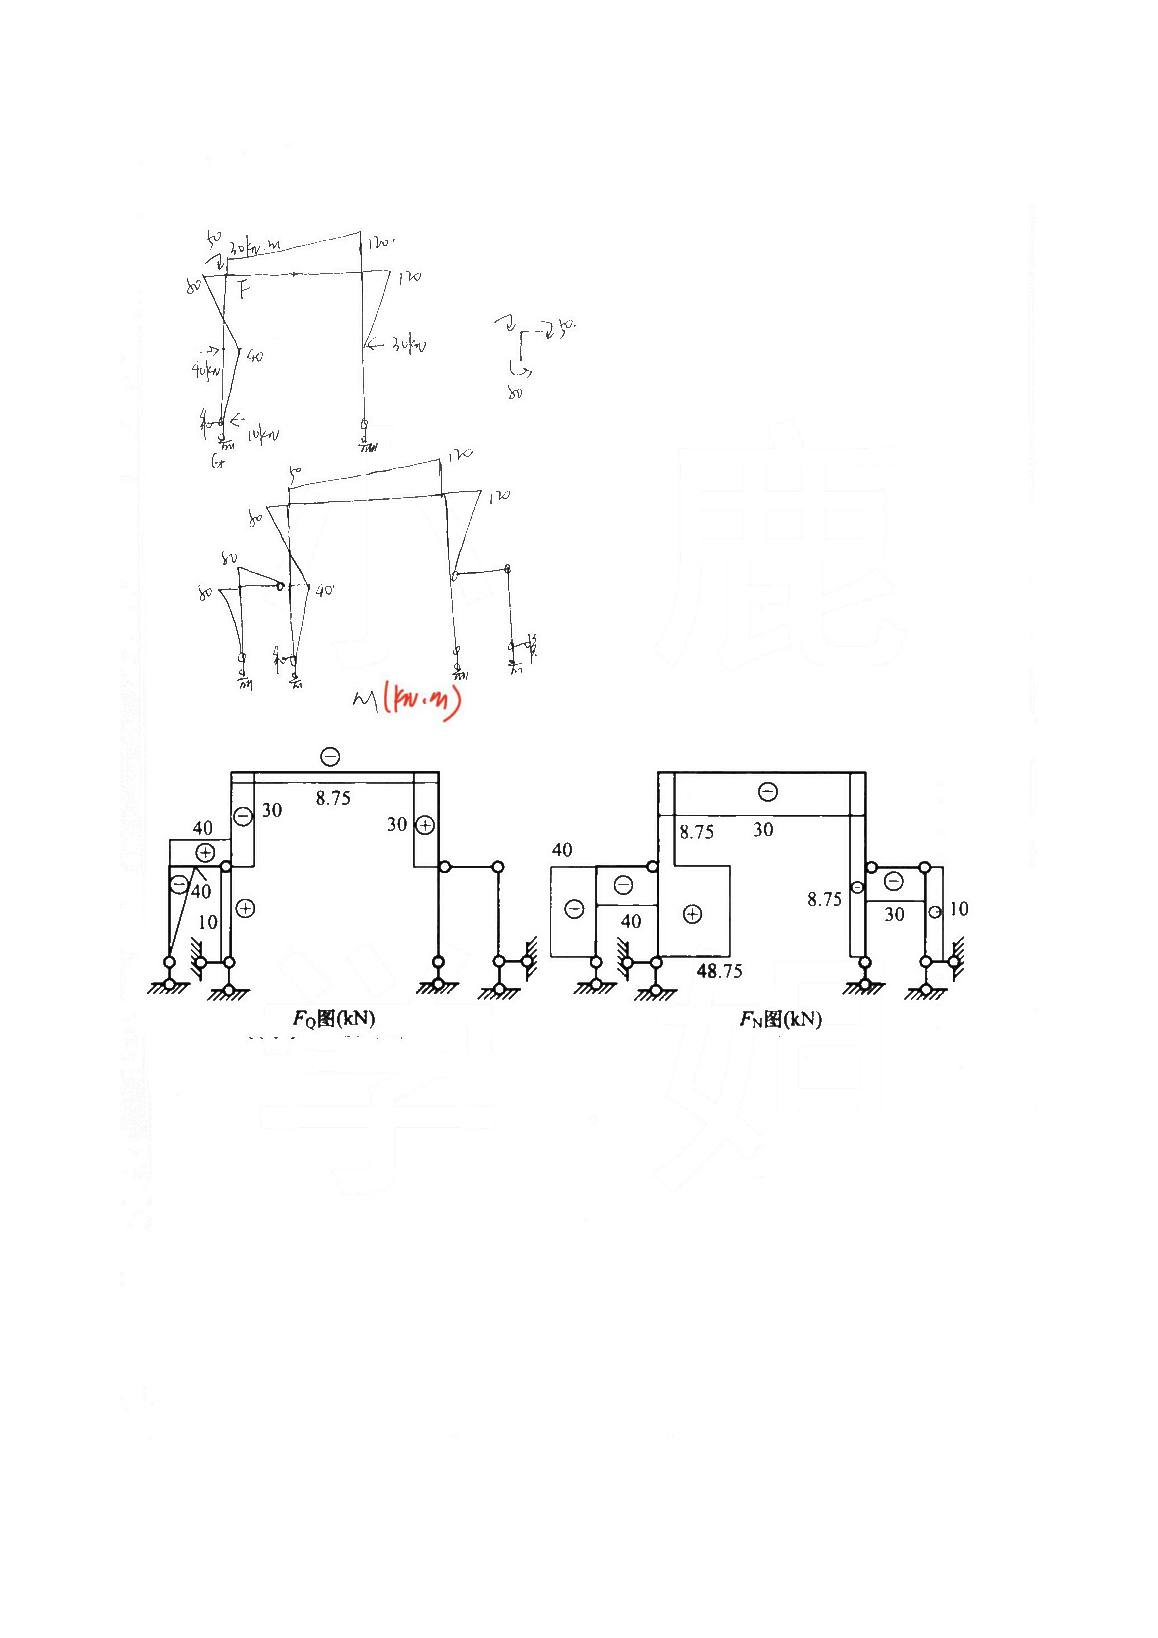
\includegraphics[width=0.92\textwidth]{figures/src07_p010.jpg}
\caption{结构力学基础与技巧班第4次作业及答案（静定梁和刚架） 第 10 页清理图形页}
\end{figure}
\subsection*{第 11 页转写}
2-6

feg

ML=MB

、Mo=Fpx=Fpq.

学姐

18

10x6x3= 180 180180
\begin{figure}[H]\centering
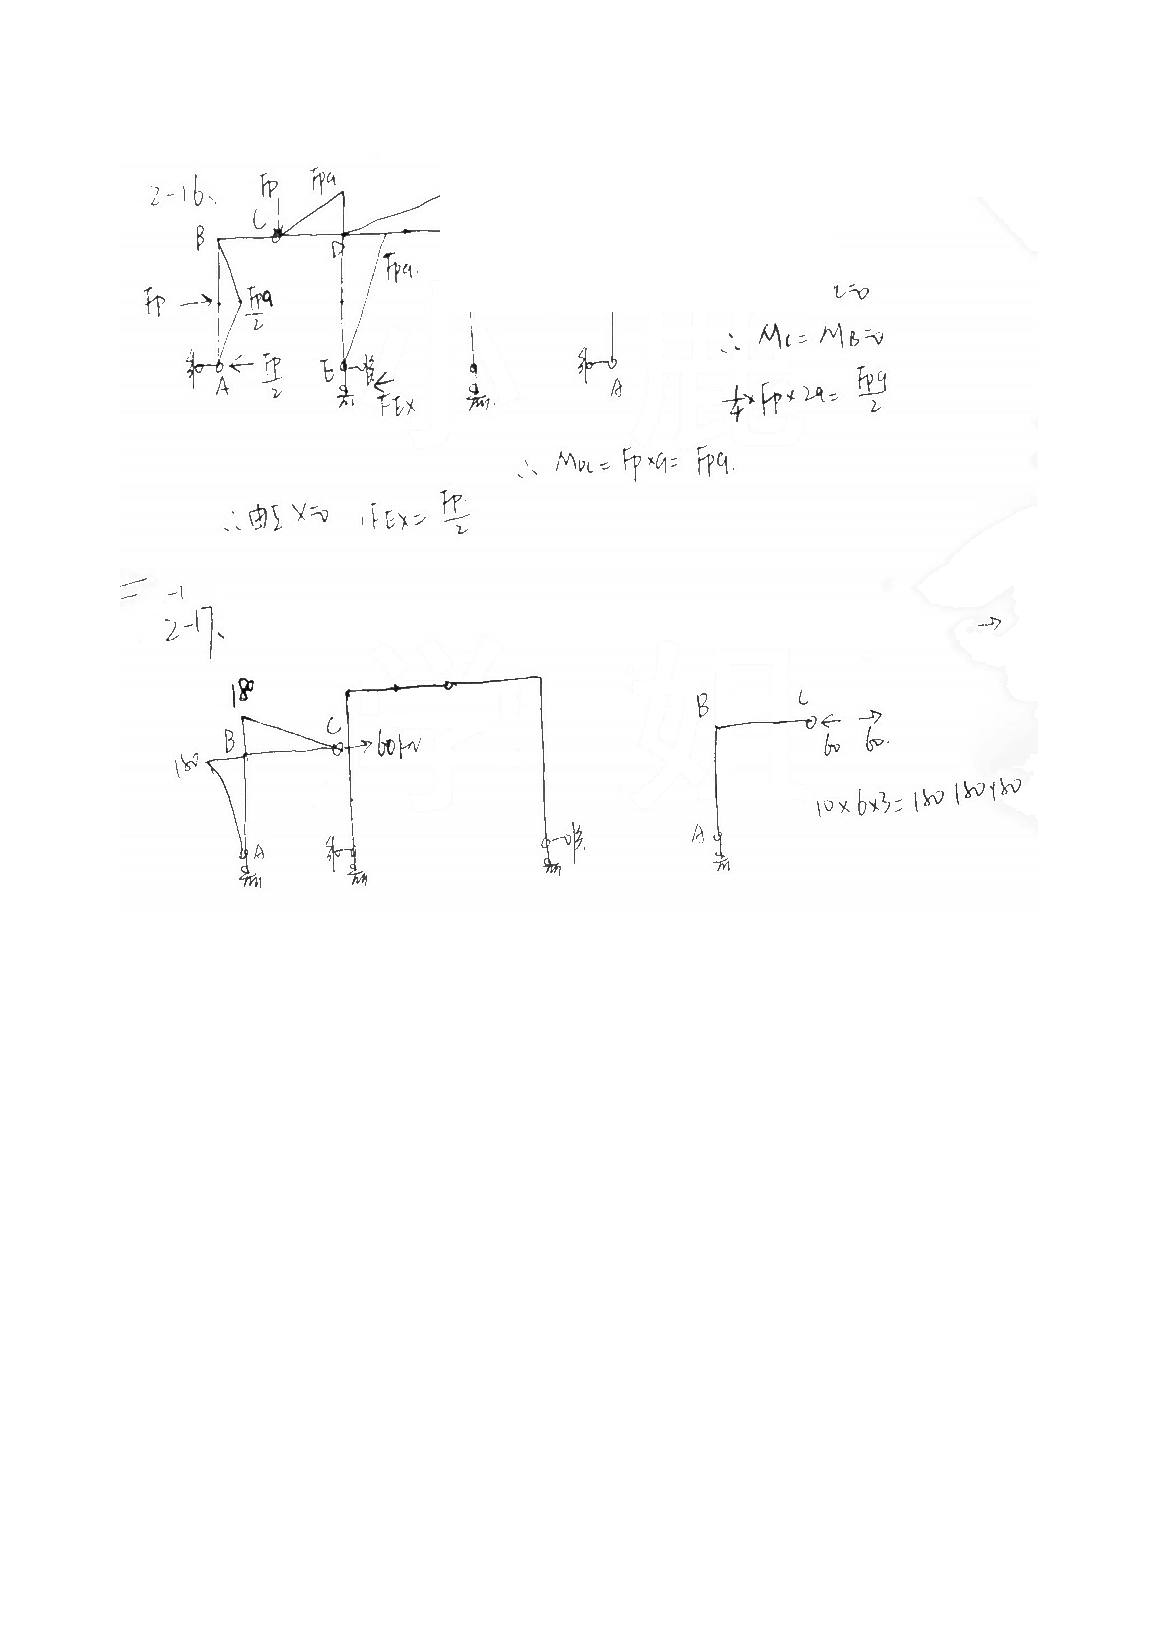
\includegraphics[width=0.92\textwidth]{figures/src07_p011.jpg}
\caption{结构力学基础与技巧班第4次作业及答案（静定梁和刚架） 第 11 页清理图形页}
\end{figure}
\subsection*{第 12 页转写}
b 1$\times$75+ 70x 12*6

70

Fryx12= bo$\times$b+ 10x3x75+ 70x 12*b

FEXEME司

X4

Frxx 9+ 70xbx3= 168. 75$\times$ 6

652-5

675

675

x- -751

652

MG= b0x3+ 10x3*号

2-8、

30

120

不统传还

chh

5FHX=5（由从4可得）

EM40

Fy$\times$4=10x4x2+5

Fay=

Zxn = *hy =+ Kei +hxxa

T3x= 75kv

x loy 4= 70.
\begin{figure}[H]\centering
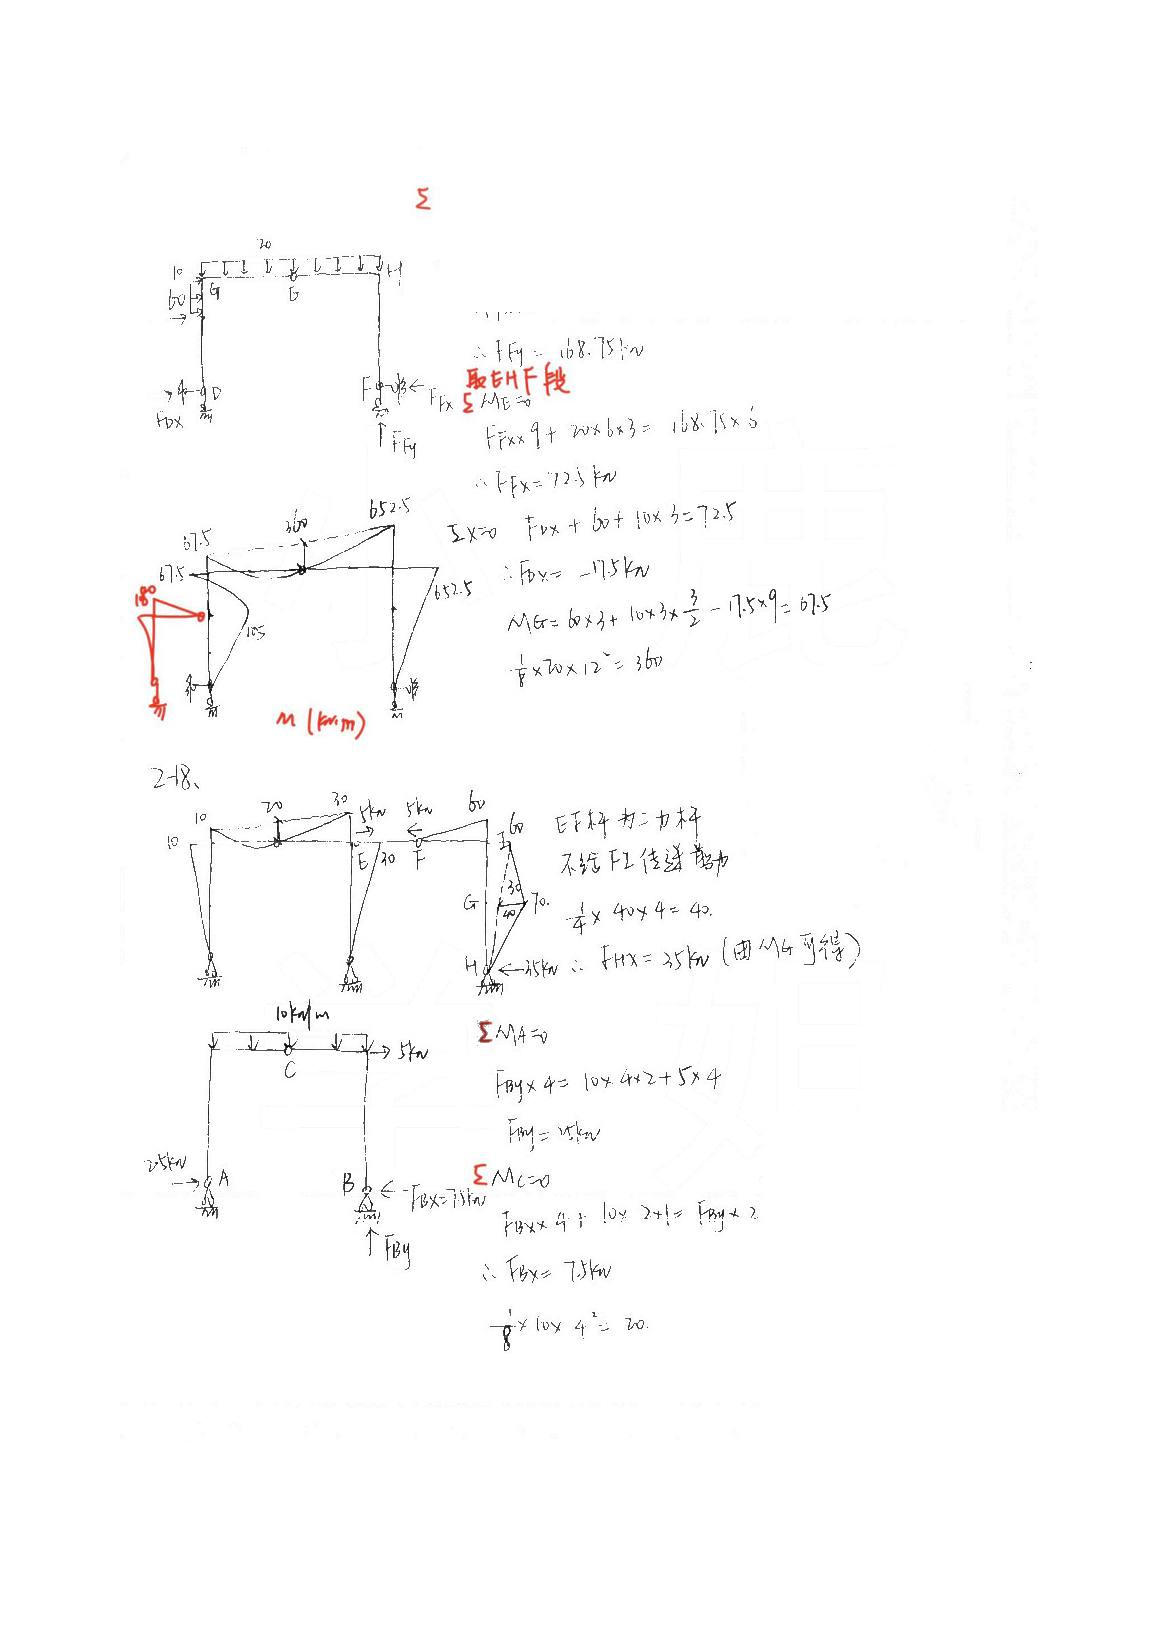
\includegraphics[width=0.92\textwidth]{figures/src07_p012.jpg}
\caption{结构力学基础与技巧班第4次作业及答案（静定梁和刚架） 第 12 页清理图形页}
\end{figure}
\subsection*{第 13 页转写}
699

2-V0.

M- m

TX$\times$ 4- 2+4423 2

FAX=2.kV

3.5

3.5

3.5

Fo图(kN)

FN图(kN)
\begin{figure}[H]\centering
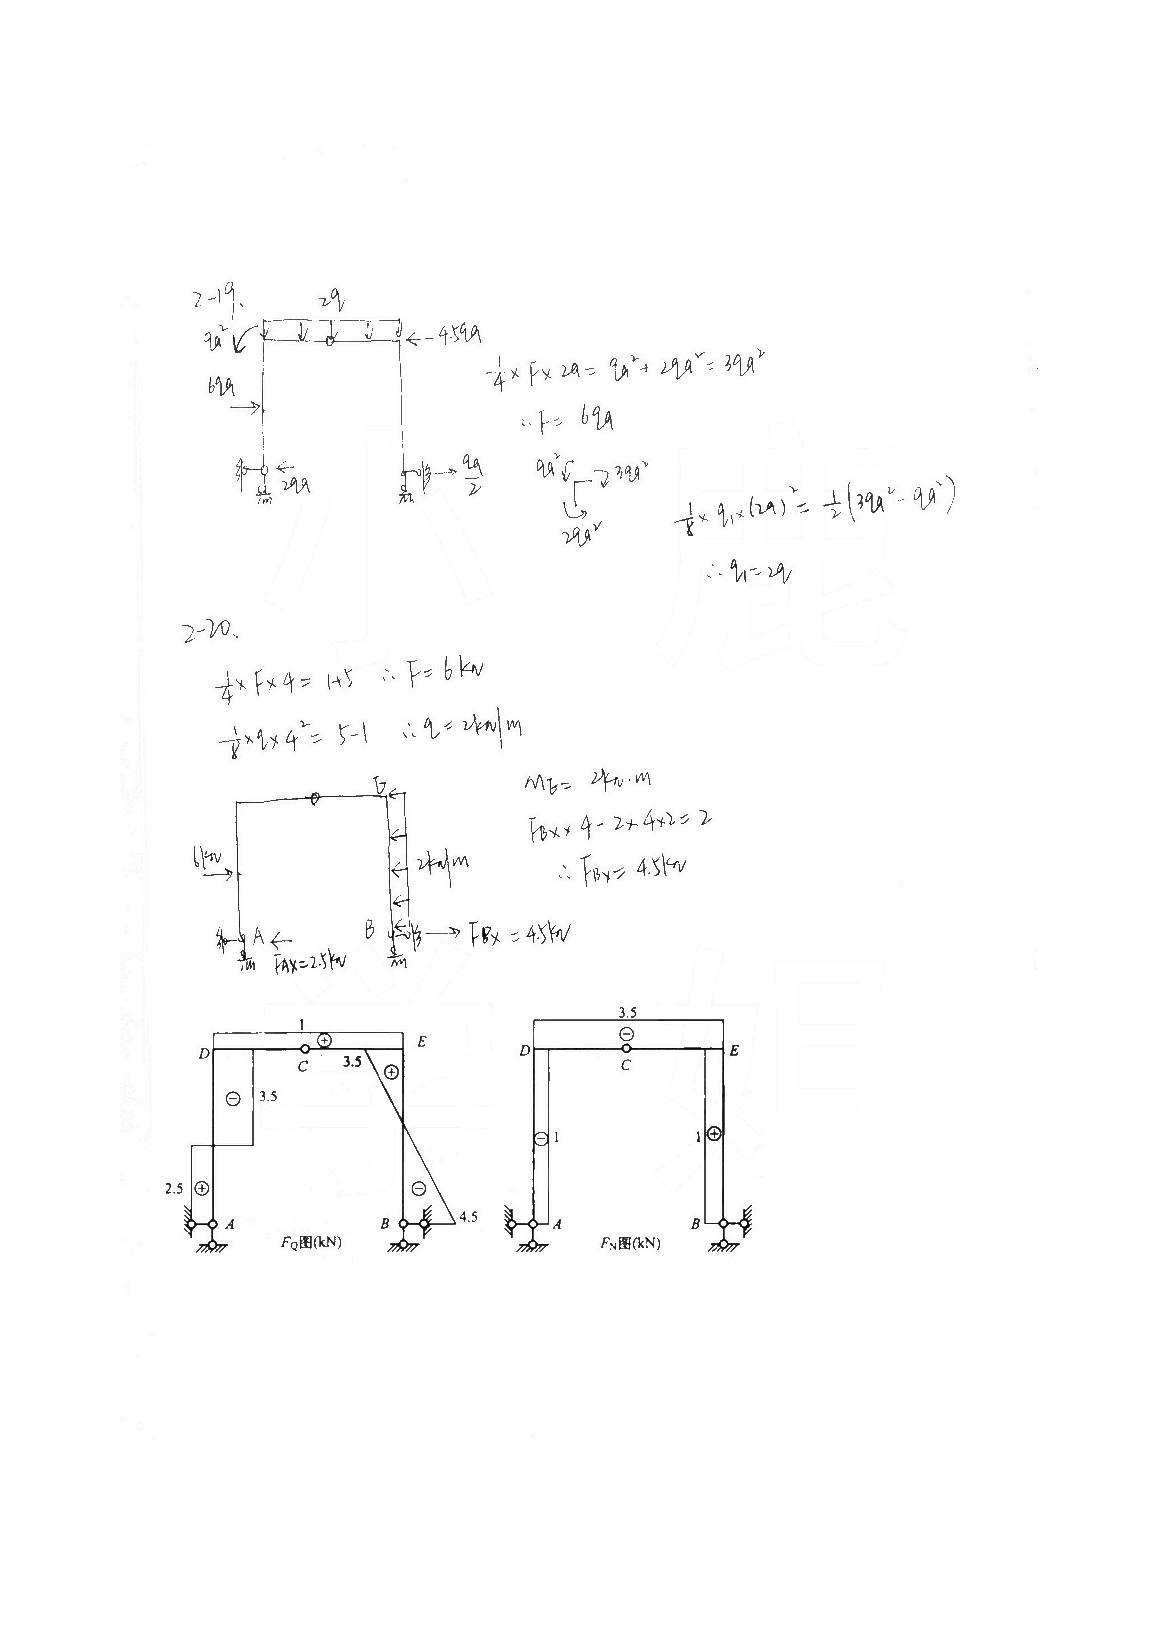
\includegraphics[width=0.92\textwidth]{figures/src07_p013.jpg}
\caption{结构力学基础与技巧班第4次作业及答案（静定梁和刚架） 第 13 页清理图形页}
\end{figure}
\subsection*{第 14 页转写}
tb

学姐4，数

环向中部传

Mr\textasciitilde{} Fpx 5\textasciitilde{} Fpx 2- 3斤
\begin{figure}[H]\centering
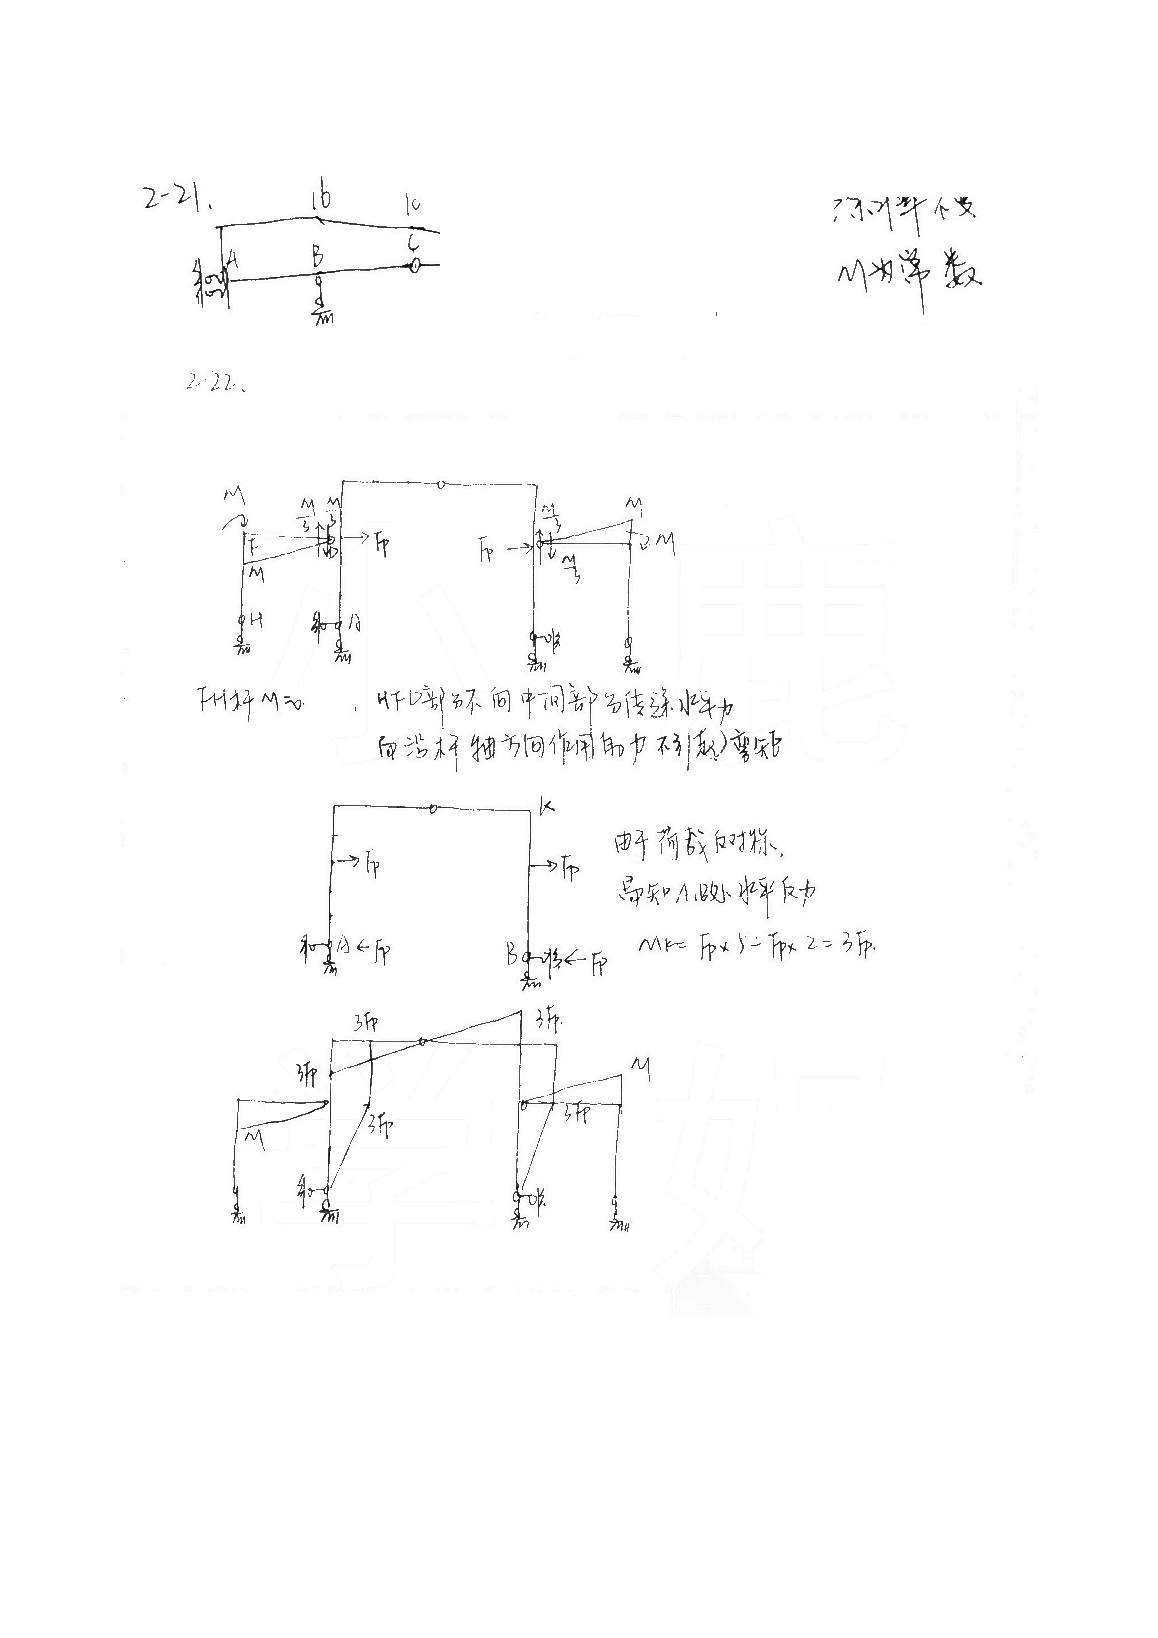
\includegraphics[width=0.92\textwidth]{figures/src07_p014.jpg}
\caption{结构力学基础与技巧班第4次作业及答案（静定梁和刚架） 第 14 页清理图形页}
\end{figure}
